\newcommand{\psd}[1]{{\small\sffamily{\color{blue!60}#1}}}

Similar simulations, as in the prvious tutorial is presented in this
section. We showcase the 2D bar problem simulation with one end clamped
wile being pulled at the other end. Contrary to simulation in the
previous tutorial, the clamped end just restricts \(x\) movement, i.e,
\(u_x=0\). Just like simulation from the prvious tutorial the body force
is neglected. Just like simulation in the prvious tutorial , the non
clamped ends pull is approximated with Neumann force
\(\int_{\partial\Omega^h_{\text N}}(\mathbf t\cdot \mathbf{v}^h)\). To
simulate the pull we assume traction vector
\(\mathbf t=[t_x,t_y]=[10^9,0]\) acting on the non clamped right end of
the bar, i.e., force in \(x\) direction is \(10^9\) units. Here is how
PSD simulation of this case can be performed.

\textbf{Step 1: Preprocessing}

For ``PSD preprocessing'' go to any folder, launch the terminal there
and run the following command.

\begin{lstlisting}[style=BashInputStyle]
PSD_PreProcess -problem linear-elasticity -dimension 2 -dirichletconditions 1 -tractionconditions 1 \
-dirichletpointconditions 1 -postprocess u
\end{lstlisting}

Additional flag \psd{ -dirichletpointconditions 1} now appears, this
notifies to PSD that there is one Dirichlet point boundary condition.
Edit the \psd{ ControlParameters.edp} to communicate the desired point
boundary conditions, set the variables \psd{ Pbc0Ux  0.} and
\psd{ Pbc0Uy  0.} to specify \(u_x=0,u_y=0\), and variable
\psd{ PbcCord = [[  0. , 0. ]];} to specify the point coordinates
\((x,y)=(0,0)\). Via the flags we specified that
\psd{ -dirichletconditions 1}, i.e., there is one Dirichlet border. To
provide the Dirichlet condition (\(u_x=0\)) set the variables
\psd{ Dbc0On 2} and \psd{ Dbc0Ux 0.} in \psd{ ControlParameters.edp}.
PSD understands that 4 is the mesh border label on which Dirichlet is
applied and (\(u_x=0\)) is the condition to be applied.

\textbf{Step 2: Solving}

Let us now use 6 cores to solve this problem. To do so enter the
following command:

\begin{lstlisting}[style=BashInputStyle]
PSD_Solve -np 6 Main.edp
\end{lstlisting}

\% Notice, that this is the exact same command used in solving the
previous bar problems from other sections, with only difference that we
now use \psd{ -np 6}.

\textbf{Step 3: Postprocessing}

Launch ParaView and have a look at the \psd{ .pvd} file in the
\psd{ PSD/Solver/VTUs\_DATE\_TIME} folder.

\begin{figure}[htbp]
    \centering
    \begin{minipage}[t][2cm][t]{0.36\textwidth}
    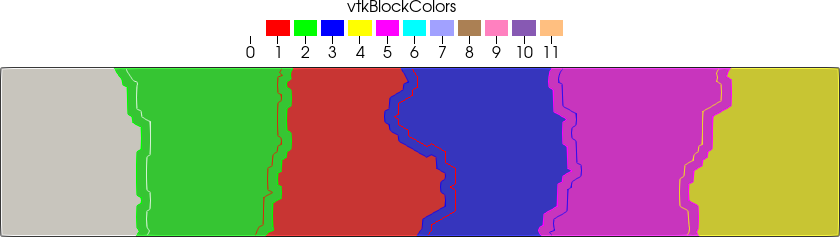
\includegraphics[align=b,width=1\textwidth]{./Images/2d-bar-partitioned6.png}
    \end{minipage}\hspace{.1\textwidth}
    \begin{minipage}[t][2cm][t]{0.5\textwidth}
    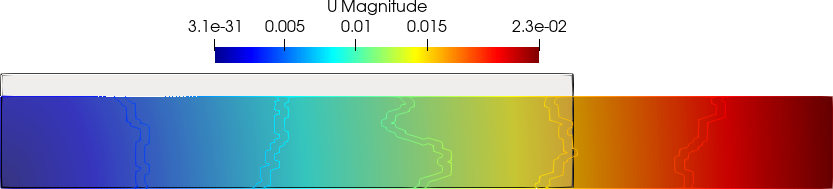
\includegraphics[align=b,width=1\textwidth]{./Images/2d-bar-clamped-traction-point.png}
    \end{minipage}
    \caption{2D bar results. Partitioned mesh (left) and 100X warped displacement field (right).}
    \label{fig:6part}
\end{figure}

Note now in\textasciitilde{}\cref{fig:6part} there are six subdomais in
the partitioned mesh. As expected, we see that the right and the left
end of the bar which is being pulled now contract in \(y\) direction,
and the bar elongates in \(x\) direction.
